\chapter{Central de procesamiento}
\section{Descripción general}
\par El diseño general del sistema se pensó como tres nodos de escucha que son comandados y
procesados por medio de una central de procesamiento. Los requerimientos de la misma se
basan en las funcionalidades para establecer una comunicación estable y segura con cada uno
de los nodos, donde en caso de detectar una inhibición por parte de cualquier nodo requerir
el estado de los otros dos para así activar las alarmas correspondientes, comunicarse al
servidor web y volver a iniciar el sistema de cero una vez que se haya terminado el proceso
correctamente, dando también un reporte del estado de salud de cada nodo en particular.
\par En este capitulo se presentará la forma en que se llevo a cabo el desarrollo de la
misma, indicando su funcionamiento, primer prototipo, diseño final y la implementación de
un gabinete. 
\subsection{Funcionamiento}
\par El funcionamiento de la misma se podría dividir en tres partes interconectadas que se detallan a continuación.
\subsubsection{Comunicación con nodos}
\todo[inline]{poner referencias a sección de comunicación rs y con sim800}
\par Como ya se detallo en el apartado \ref{com_rs485}, la comunicación optada para la interconexión de los 4 dispositivos es RS485 por su forma de transmisión diferencial y largo alcance. 
\par Al inicio del sistema la central (funcionando como el maestro en la comunicación) requiere el estado de cada uno, del cual si detecta una inhibición alguno de ellos comenzaría el proceso para ver los demás nodos y comenzar a activar alarmas.

\subsubsection{Alarmas locales}
\par Una vez detectada la inhibición y procesado el estado del sistema en general, se dan las alarmas visuales y sonoras en la central misma para dar aviso al personal de seguridad que se encuentra en el lugar. 

\subsubsection{Comunicación remota al servidor web}
\par Como ya vimos en el apartado \ref{sim800}, la comunicación con el servidor web se hace de manera remota mediante GPRS una vez que se encuentra el sistema en un estado de alarma, cargando en el mismo la ubicación, ID de nodos, entre otros que se detallaran en las siguientes secciones. 

\section{Prototipo}
\subsection{Diseño}
\subsubsection{PCB}
\par En la figura \ref{im:pcb-prototipo} podemos ver una vista superior (izquierda) e inferior (derecha) de la placa prototipo para llevar a cabo la implementación de esta. 
\begin{figure}[h!]
\begin{center}
    \subfigure{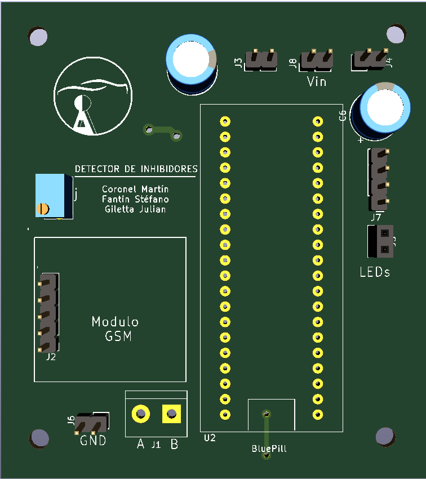
\includegraphics[width=60mm]{images/central/placa-prot-central-superior.png}}
    \subfigure{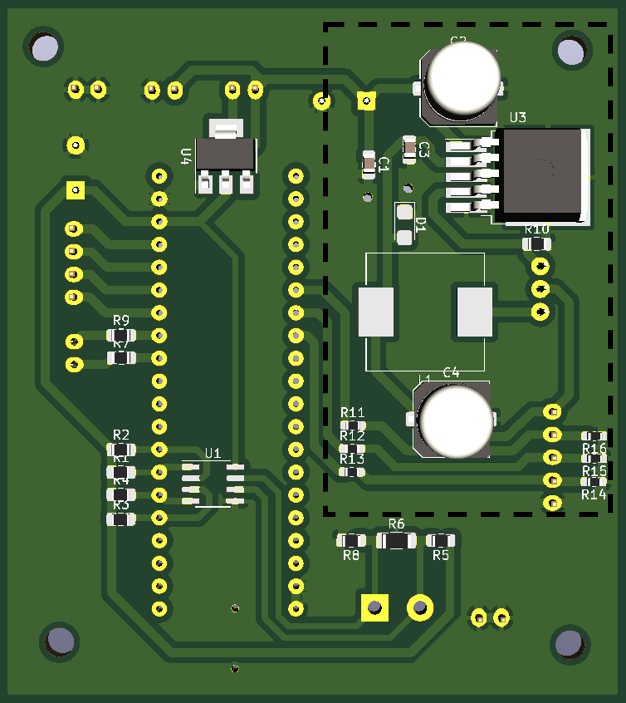
\includegraphics[width=60mm]{images/central/placa-prot-central-inferior.png}}
    \caption{Prototipo de placa de la central de procesamiento.}
	\label{im:pcb-prototipo}
\end{center}
\end{figure}

\subsection{Problemas surgidos}
\par Los principales problemas de esta primera aproximación al diseño final fueron en
base a la alimentación requeridas por el integrado de comunicación GPRS.
\par En primer lugar, era necesario un capacitor en la alimentación del SIM800 para
suavizar el arranque del mismo, ya que al conectarse a una red GSM/GPRS requiere un pico
de corriente de 2A.
\par Por otra parte, al tener que rediseñar la placa, notamos que la fuente conmutada implementada (encerrada en lineas cortadas en la figura \ref{im:pcb-prototipo}) requería gran cantidad de componentes, aumentando así el costo, principalmente con el integrado e inductor necesarios. Por ello, se opto como solución un regulador lineal con tan solo dos capacitores y dos resistencias se obtienen los requerimientos pedidos. 

\section{Diseño final}
\subsection{Software}
\par Para no volver redundante la explicación respecto del prototipo, se opto que el
funcionamiento del sistema embebido se detalle en esta sección ya que en cuanto a este no
fueron grandes los cambios realizados. 

\begin{figure}[h!]
	\centering
	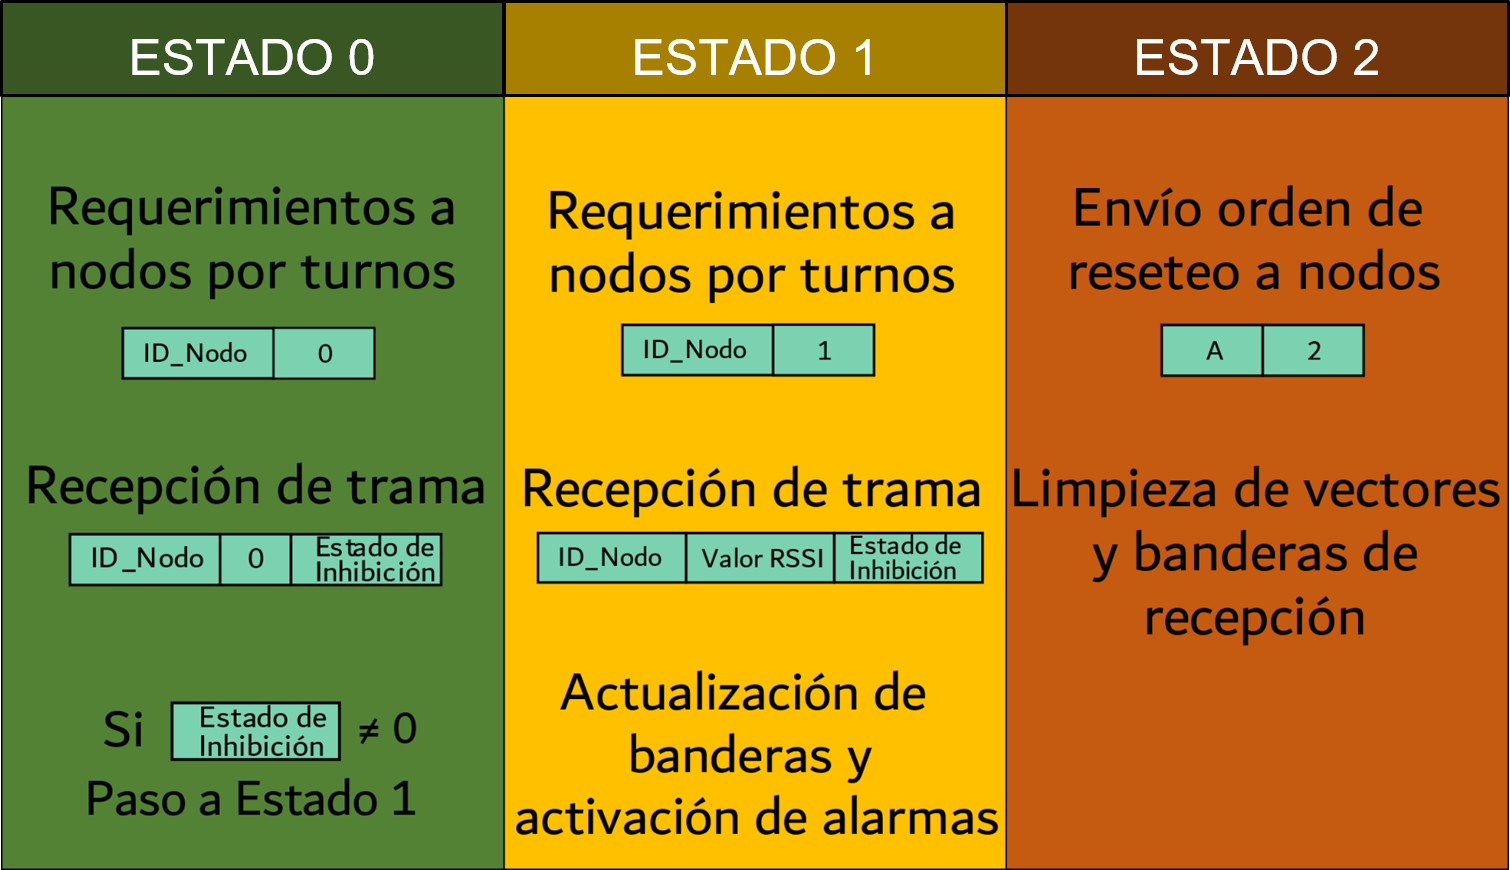
\includegraphics[scale=.53]{images/central/maquina-estado-central.png}
    \caption{Estados de la central en comunicación con nodos.}
	\label{im:maq-est-central}
\end{figure}

\subsection{Hardware}
\subsubsection{Esquemático}
\subsubsection{PCB}
\subsubsection{Modelo 3D}
\section{Gabinete}
\par El diseño del gabinete (figura \ref{im:gabinete-central}) de la central se busco que fuera de una forma vertical, en donde por delante se observen cinco indicadores lumínicos que informar sobre el estado de inhibición del sistema (agregado de un buzzer también), el estado de salud de cada nodo y si esta en funcionamiento o no.
\par Por la parte trasera encontramos un interruptor para alimentar a todos los nodos, conector para 12V y un conector GXS para la comunicación RS485 y llevar la alimentación a cada nodo bajo el concepto de power over ethernet. 
\begin{figure}[h!]
\begin{center}
    \subfigure{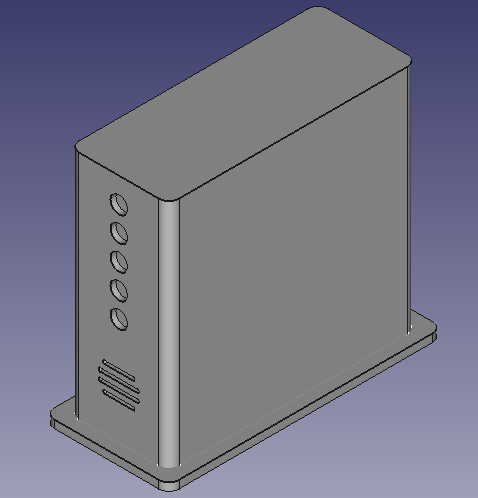
\includegraphics[width=60mm]{images/central/modelo-3d-central-frente.png}}
    \subfigure{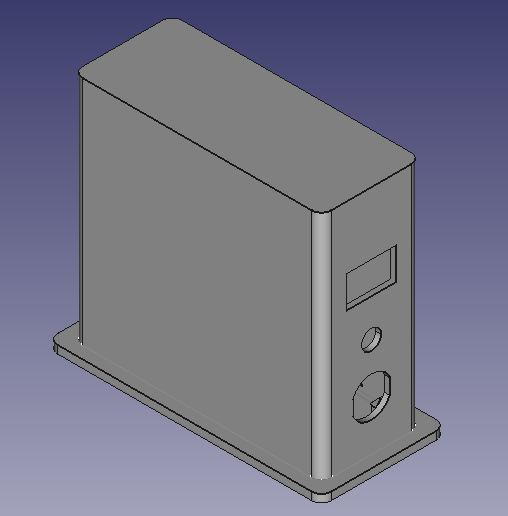
\includegraphics[width=61.5mm]{images/central/modelo-3d-central-atras.png}}
    \caption{Gabinete de central armado.}
	\label{im:gabinete-central}
\end{center}
\end{figure}

\par El mismo se llevo a la realidad por medio de impresión 3D en plástico PLA negro. Para comodidad en el armado e impresión, vemos en la figura \ref{im:impresion-central} que el modelo se dividió en 2 partes, donde una llamada "base" es la encargada de soportar la placa principal de la central y en la parte de la derecha, que denominamos "tapa", encontramos los indicadores y demás conectores. 

\begin{figure}[h!]
	\centering
	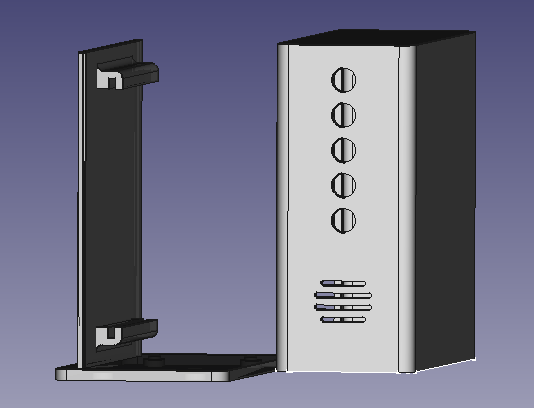
\includegraphics[scale=.53]{images/central/modelo-3d-central-separado.png}
    \caption{Partes para el armado del gabinete de central.}
	\label{im:impresion-central}
\end{figure}
